% arXiv entry point: public author version with the appendix included.
% Keep this as the only .tex file in the upload so AutoTeX has one root.
\pdfoutput=1
\def\ICLRArxivVersion{1}
\def\ICLRIncludeAppendix{1}
\pdfminorversion=7
\documentclass{article} % For LaTeX2e
\usepackage{iclr2027_conference,times}

% Optional math commands from https://github.com/goodfeli/dlbook_notation.
\input{math_commands.inc}

\usepackage{algorithm}
\usepackage{algpseudocode}
\ifdefined\ICLRIncludeAppendix
\else
\usepackage{xr-hyper}
\fi
\usepackage[hidelinks]{hyperref}
\ifdefined\ICLRIncludeAppendix
\else
\externaldocument[][nocite]{appendix}
\fi
\usepackage{url}
\Urlmuskip=0mu plus 2mu\relax
\def\UrlBreaks{\do\/\do\-\do\.\do\_\do\?\do\&\do\=}
\usepackage{graphicx}
\usepackage{booktabs}
\usepackage{array}
\usepackage{longtable}
\usepackage{float}
\usepackage{multirow}
\usepackage{xcolor}
\usepackage[section]{placeins}
\newcolumntype{P}[1]{>{\raggedright\arraybackslash}p{#1}}
\setlength{\emergencystretch}{1.5em}

\title{Beyond Correctness: Evaluating Semantic Knowledge in Cross-Table Transfer}
\ifdefined\ICLRArxivVersion
\author{\normalfont
\textbf{Seokyong Sheem}\thanks{Equal contribution.} \quad \textbf{Hochang Lee}\footnotemark[1] \quad \textbf{Suyeong Lee} \quad \textbf{Daekyum Kim}\thanks{Corresponding author.} \\
Korea University \\
\texttt{\{sheemsy, cvcvcv99, tsw1615, daekyum\}@korea.ac.kr}
}
\else
\author{Anonymous Authors}
\fi


% Review submission: leave commented
%\iclrfinalcopy
\ifdefined\ICLRArxivVersion
\iclrfinalcopy
\fi

\newcommand{\fix}{\marginpar{FIX}}
\newcommand{\new}{\marginpar{NEW}}
\newcommand{\Ksupplied}{K^{\mathrm S}}
\newcommand{\Kaltered}{K^{\mathrm A}}
\newcommand{\Kref}{K^{0}}
\newcommand{\supp}[1]{\textnormal{Supp.~#1}}
\usepackage{enumitem}
% \newcommand{\suppref}[1]{the supplement's \emph{#1}}

\begin{document}

\maketitle
\ifdefined\ICLRArxivVersion
\lhead{}
\fi
\begin{abstract}

Semantic knowledge is increasingly used to bridge heterogeneous schemas in tabular learning, but how much does that knowledge actually improve prediction?
Studies in tabular learning commonly answer this question through semantic ablations that modify or suppress the supplied semantic knowledge.
We show that these ablations can lead to misleading conclusions about predictive benefit: poor performance under altered semantics may be taken as evidence that the intended knowledge is beneficial.
Across real and controlled experiments, altering semantic content can produce large performance differences even when the model gains little predictive benefit from having that semantic knowledge in the first place.
To separate these effects, we distinguish two quantities: content sensitivity and predictive utility. 
Content sensitivity measures the change in performance when semantic content is altered, whereas predictive utility measures the benefit of the intended semantic knowledge relative to a suitable reference without that knowledge.
This distinction motivates an evaluation framework in which the control is chosen according to the question being asked: altered controls assess sensitivity to semantic content, whereas claims that semantic knowledge improves prediction require a suitable reference.
Even then, predictive utility is not fixed; it varies across suitable references and decreases when the reference can more easily recover the tested knowledge from other inputs or labeled examples.
In a bounded audit of 25 semantic-ablation comparisons across nine studies, only one of 18 explicit predictive-utility claims is paired with a control that clearly isolates the tested semantic contribution.
Together, these findings motivate a simple evaluation principle: semantic-ablation controls should be chosen and interpreted according to the question they are intended to answer. 

Code and reproducibility artifacts are available at \url{https://github.com/mintlabkorea/beyond-correctness}.

\end{abstract}

\section{Introduction}

% P1. 
While tabular datasets record data in a structured format, they often organize similar information under different schemas. 
Across datasets, corresponding variables may differ in their names, coding conventions, units, scales, or measurement protocols, even when they represent the same underlying concept. 
Predictive models typically rely on schema-specific input representations, making direct transfer difficult when the source and target schemas differ. 

Recent approaches to cross-table transfer and pretrained tabular learning increasingly leverage semantic knowledge to interpret heterogeneous schemas and enable transfer across datasets \citep{wang2022transtab,kim2024carte,kim2025tarte,arazi2025tabstar}.
Such knowledge can come from feature names, dataset documentation, codebooks, knowledge graphs, or domain rules, and can help interpret recorded values, identify corresponding variables, and introduce structured relationships useful for prediction \citep{pang2015biobankconnect,li2025harmonization,ruiz2023plato,han2024featllm}.
As such knowledge becomes increasingly integrated into tabular learning, it becomes important to determine how much the supplied knowledge contributes to predictive performance. 

% P2. 
Studies in tabular learning commonly address this question through semantic ablations that modify or suppress the supplied semantic knowledge \citep{dinh2022lift,hegselmann2023tabllm}.
For example, feature names or other semantic inputs may be shuffled, permuted, anonymized, or omitted, and the resulting performance is compared with that obtained using the intended semantic knowledge \citep{dinh2022lift,hegselmann2023tabllm}.
However, differences in performance between intended and altered condition does not necessarily mean that the intended knowledge improves prediction \citep{hewitt2019designing,elazar2021amnesic,sturmfels2020visualizing}.
Such differences can arise when changing the semantic content reduces performance in the altered condition.
The resulting performance gap therefore does not isolate the benefit of the intended knowledge, as it also captures degradation from the altered condition.
In such cases, the ablation may be misinterpreted as showing that the intended semantic knowledge improves prediction relative to a condition without that knowledge.

% P3. 
To separate these effects, we distinguish two evaluation quantities: content sensitivity and predictive utility. 
Content sensitivity measures how performance changes when the supplied semantic content is altered, whereas predictive utility measures the benefit of the intended semantic knowledge relative to a suitable reference in which the tested component is unavailable. 
The two quantities answer different questions: content sensitivity asks whether prediction depends on which semantic content is supplied, whereas predictive utility asks whether having the tested knowledge improves prediction in the first place.
Evaluating predictive utility therefore requires a suitable reference that satisfies three criteria: (1) Removal: remove the tested semantic component; (2) Preservation: preserve all other model inputs and how they are presented; and (3) Setup: keep the model and learning procedure unchanged.
% A suitable reference must remove the tested semantic component while preserving all other model inputs, their representation, and the model and learning procedure. 
This leads to a claim-matched evaluation principle: the control should be chosen according to the question the comparison is intended to answer.

\begin{figure}[t]
\centering
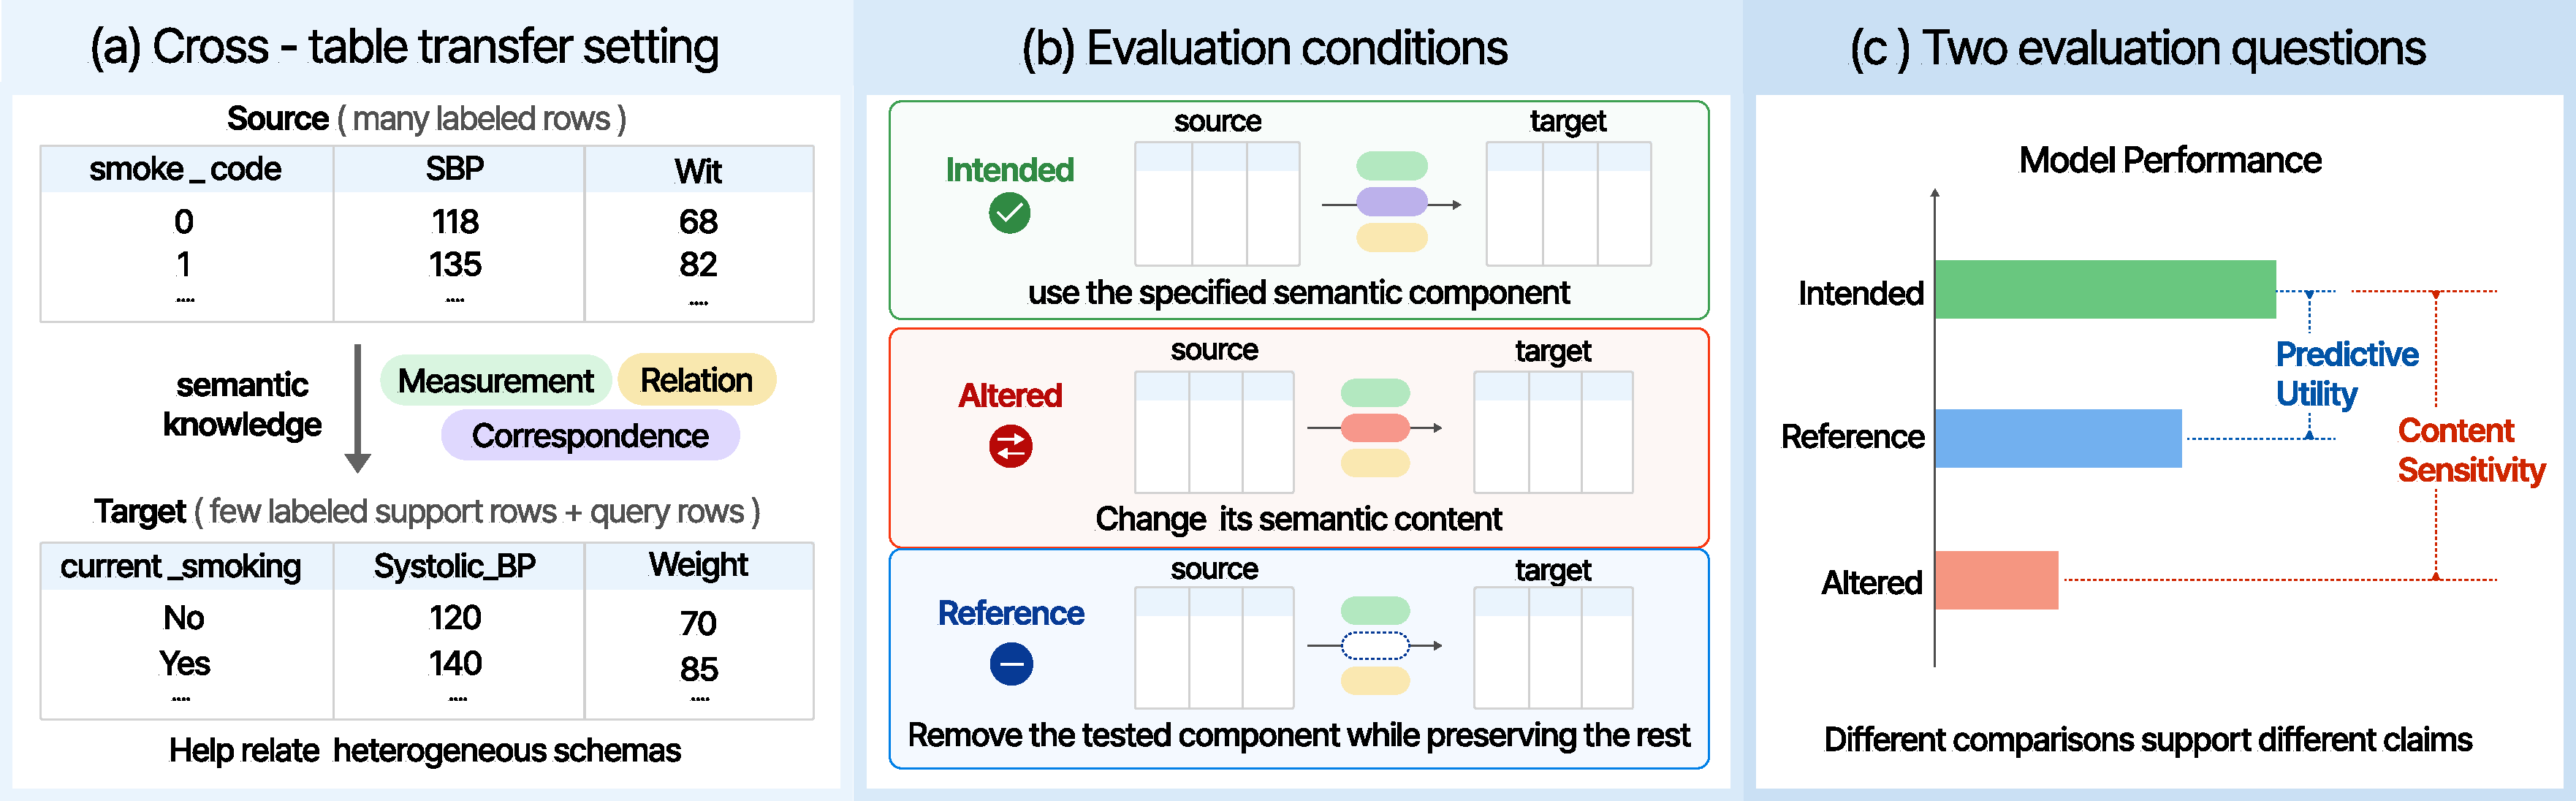
\includegraphics[width=\linewidth]{overview.pdf}
\caption{
\textbf{Overview of the evaluation framework.}
(a) Semantic knowledge relates heterogeneous source and target schemas.
(b) The intended condition uses the specified content, the altered condition changes it, and the reference removes the tested component while preserving the remaining setup.
(c) Intended--altered measures \emph{content sensitivity}, whereas intended--reference measures \emph{predictive utility}; the two comparisons support different claims.
}

\label{fig:overview}
\vspace{-10pt}

\end{figure}

% P4. Findings 
Our experiments show that these distinctions matter in practice. 
Across an existing semantic tabular model, real cross-table transfer tasks, and controlled experiments, altering semantic content can produce large performance differences even when the intended knowledge provides little predictive benefit over a suitable reference. 
In several settings, much of the intended–altered difference is explained by degradation under the altered condition rather than improvement attributable to the intended knowledge. 
The effect is not resolved simply by choosing a suitable reference: predictive utility itself varies across suitable references and decreases when the reference can more easily recover the tested information from other observed inputs or labeled target examples. 
Thus, the measured benefit depends not only on the knowledge being evaluated, but also on what the comparison condition can recover without it.

The same issue is visible in published practice. 
In a bounded audit of 25 semantic-ablation comparisons across nine studies, only one of 18 explicit predictive-utility claims is paired with a control satisfying all three requirements for a suitable reference; 11 fail at least one requirement and six are indeterminate from the published description. 
This does not imply that the corresponding semantic knowledge is unhelpful.
Rather, it means that the reported comparison does not by itself isolate the claimed predictive utility. 
Together, these findings motivate evaluation designs in which semantic-ablation controls are selected and interpreted according to the question they are intended to answer.  

\noindent\textbf{Contributions.}
\begin{itemize}[leftmargin=1.2em, labelsep=0.4em,
                itemsep=1pt, topsep=1pt, parsep=0pt, partopsep=0pt]

\item \textbf{Conceptual.} 
We show that semantic-ablation effects can conflate predictive benefit with degradation induced by the control, and distinguish content sensitivity from predictive utility to separate these effects. 
\item \textbf{Methodological.} 
We propose claim-matched evaluation with criteria for constructing suitable references and for assessing sensitivity to the choice of reference.  
\item \textbf{Empirical.} 
Through a reanalysis of an existing semantic tabular model, real cross-table transfer tasks, controlled experiments, and published ablations, we identify when and why semantic-ablation effects diverge from predictive utility and how measured utility changes with the information available to the reference. 

\end{itemize}

\section{Related Work}

\subsection{Semantic Knowledge in Cross-Table Transfer}

Cross-table methods such as TransTab and CARTE use semantic knowledge to relate heterogeneous schemas: TransTab incorporates feature descriptions, while CARTE uses open-vocabulary representations \citep{wang2022transtab,kim2024carte}. Related semantic tabular methods, such as TabLLM, serialize feature names and values as text \citep{hegselmann2023tabllm}.
More broadly, semantic or structured information in tabular learning can come from dataset documentation, schema-matching systems, knowledge graphs, language-model-generated features and rules, or task-derived behavioral constraints \citep{pang2015biobankconnect,li2025harmonization,ruiz2023plato,han2024featllm,kim2025kinematics}.
These works primarily study how such information is obtained, represented, or used, leaving open whether a particular use improves prediction.

\subsection{Evaluating the Contribution of Semantic Knowledge}

Across semantic tabular learning, ablations often compare standard semantic inputs with altered alternatives, such as shuffled or permuted inputs, or with omission-based controls, as in LIFT and TabLLM \citep{dinh2022lift,hegselmann2023tabllm}.
Because these controls can change different aspects of the input, a performance gap may reflect more than the contribution of the tested semantic knowledge.
Related work on probing, information removal, and attribution similarly shows that conclusions depend on what a control changes, what it keeps fixed, and the chosen reference point \citep{hewitt2019designing,fisher2019all,elazar2021amnesic,sturmfels2020visualizing}.
Separately, transfer-learning studies show that the value of transferred information can diminish as labeled target support increases \citep{he2019rethinking,tripuraneni2020theory,zoph2020rethinking,nguyen2020leep}.
We therefore evaluate semantic interventions using claim-matched controls, distinguishing sensitivity to semantic content from predictive utility relative to a suitable reference and examining how utility varies across suitable references.

\section{Evaluating the Contribution of Semantic Knowledge}
\label{sec:method}

\subsection{Evaluation Design}
\label{sec:evaluation_design}

We evaluate each semantic component under matched conditions, holding the evaluation data, model, training procedure, and all other components fixed.
Our experiments use a labeled source table and a target table, with labeled target rows for adaptation and the remaining rows for evaluation.
In the TabLLM reanalysis, semantic knowledge is instead varied within the model input.

We study three recurring roles of semantic knowledge.
\emph{Measurement} knowledge interprets coding, polarity, scales, units, and missing-value meanings;
\emph{correspondence} knowledge identifies compatible variables across schemas;
and \emph{relation} knowledge specifies structure among variables, such as derived values or directional constraints.
These roles organize the test cases and are not treated as a full taxonomy.

For each component, the \emph{intended condition} uses its prespecified form.
We use \emph{control} as a general term for a condition against which the intended condition is compared.
An \emph{altered control} changes the tested semantic content while preserving how it is used in prediction, whereas a \emph{removal control} omits that content.
A removal control serves as a \emph{suitable reference} only if it satisfies the criteria in Section~\ref{sec:reference}.
Let $Q_c$ denote performance under condition $c$.
All conditions use the same evaluation rows and procedure, and higher is better for every metric.
We define

\begin{align}
\text{Predictive utility}
    &= Q_{\mathrm{intended}} - Q_{\mathrm{reference}},\\
\text{Content sensitivity}
    &= Q_{\mathrm{intended}} - Q_{\mathrm{altered}}.
\end{align}

\begin{table}[h]
\caption{Condition construction for measurement, correspondence, and relation knowledge.}
\label{tab:knowledge_conditions}
\centering
\fontsize{8pt}{9pt}\selectfont
\setlength{\tabcolsep}{3pt}
\renewcommand{\arraystretch}{0.92}

\begin{tabular}{@{}P{0.16\linewidth}P{0.25\linewidth}P{0.29\linewidth}P{0.25\linewidth}@{}}
\toprule
Knowledge & Intended & Altered & Reference \\
\midrule

Measurement &
Specified coding or numerical conversion &
Altered coding or numerical conversion &
Raw source values \\

Correspondence &
Specified source--target pairing &
Permuted source--target pairing &
No shared pairing; separate source and target columns \\

Relation &
Specified relation and direction &
Reversed direction or random relation &
No added value or constraint \\

\bottomrule
\end{tabular}
\end{table}

For correspondence, the reference keeps the same number of columns but places source and target values in separate columns rather than a shared matched column.
In the controlled benchmark, known schema transformations define the intended measurement and correspondence knowledge, while the synthetic outcome mechanism defines the intended relations.
In real-data experiments, intended knowledge is derived from documentation or domain sources before evaluation and is not assumed to be ground-truth correct.

\subsection{Constructing a Reference}
\label{sec:reference}

A suitable reference must remove the evaluated semantic component while preserving the rest of the comparison.
Simply removing the component may also change the input; for example, removing feature names can turn a key--value input into a values-only input (Figure~\ref{fig:reference_construction}).

Removing the evaluated component yields a candidate reference, which is suitable only if it satisfies three criteria:
(i) \emph{Removal}: it removes the evaluated semantic component;
(ii) \emph{Preservation}: preserves all other information available to the model and how that information is presented, including feature identity, input width, and format;
(iii) \emph{Setup}: leaves the model, learning procedure, and other modeling choices unchanged.

\begin{figure}[h]
\centering
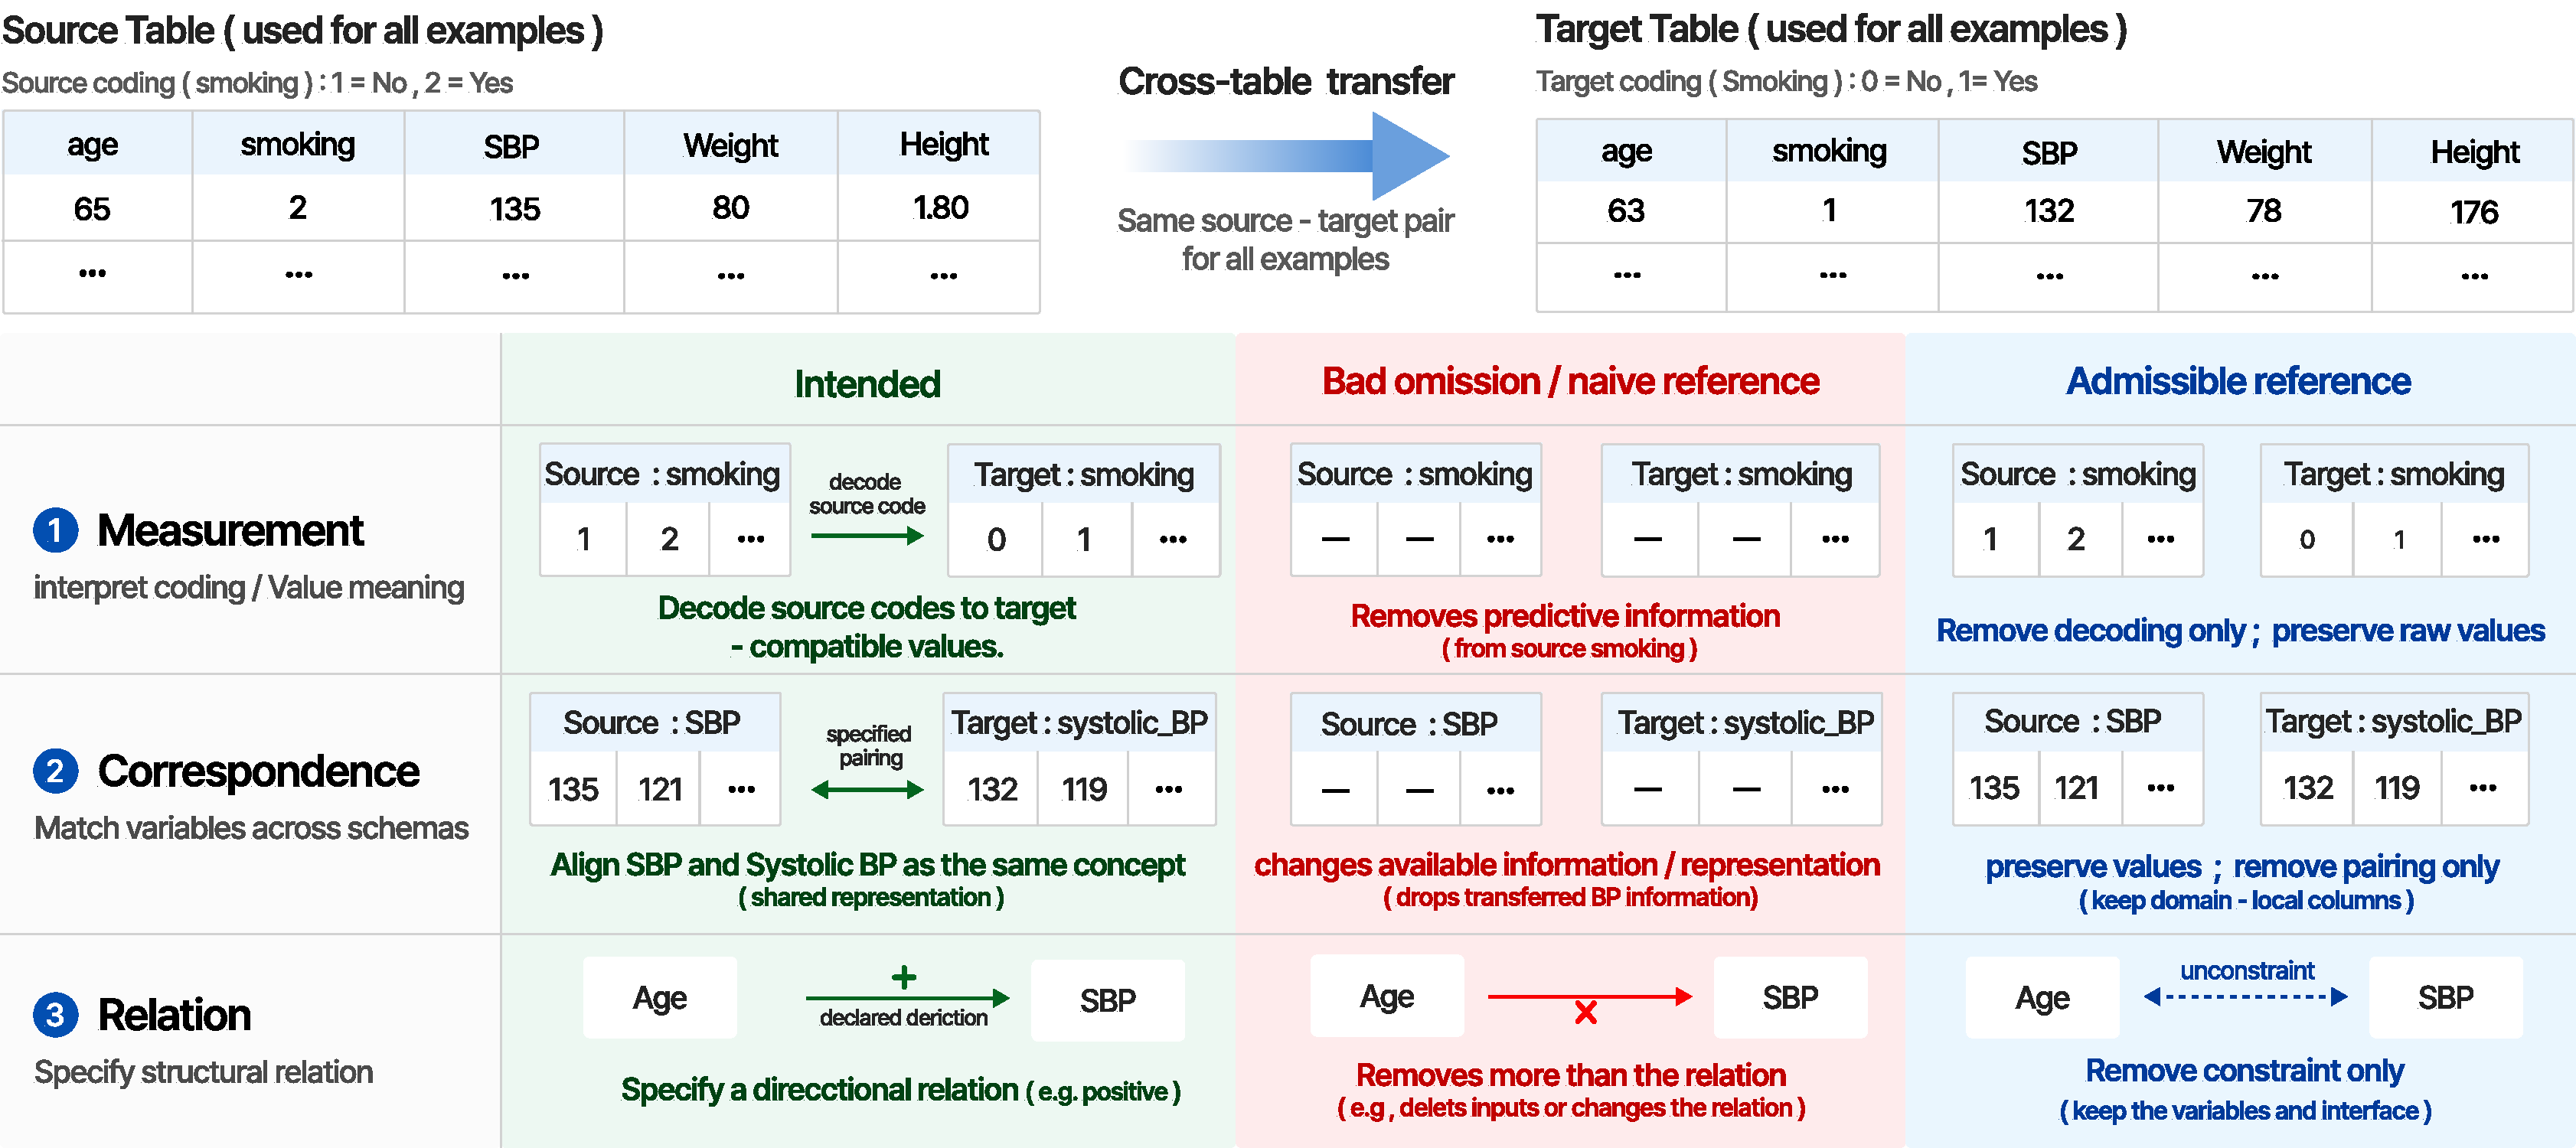
\includegraphics[width=0.9\linewidth]{method.pdf}
\caption{
\textbf{Suitable and unsuitable references for the three roles of semantic knowledge. }
Suitable references remove only the tested component while preserving the remaining predictive information and setup. 
Unsuitable controls either remove additional predictive information or alter, rather than remove, the tested component.
}
\label{fig:reference_construction}
\end{figure}

For text inputs, changing the tested text can change tokens; this alone does not fail Preservation. 
For feature-name tests, Removal means that the original feature-name meaning is removed; we do not assume that every anonymous label has exactly the same effect on the model.
In the published-ablation audit, we check Preservation by asking whether the other predictive values, feature identity, input width, and the rest of the input format are preserved, and check Setup by asking whether the model and learning procedure are unchanged \supp{\S\ref{sec:published_audit}}.

Controls that fail these criteria may support broader comparisons but do not isolate predictive utility.
Predictive utility is defined relative to a particular suitable reference, so different suitable references need not give the same value.
If multiple references satisfy these criteria, we report reference sensitivity; if none does, predictive utility is not separately evaluable.

For a specified suitable reference, predictive utility is positive or negative when its 95\% confidence interval lies entirely above or below zero; otherwise it is unresolved.
Thus, \emph{not separately evaluable} means that no suitable reference exists, whereas \emph{unresolved} means that a suitable reference exists but the effect direction is not resolved.
Resolution diagnostics are reported in \supp{\S\ref{sec:app-controlled-boundaries}}.

In practice, claim-matched evaluation states the claim, selects a matching altered or removal control, and, for predictive utility, verifies Removal, Preservation, and Setup before reporting the contrast.

\subsection{Constructing Semantic Knowledge}
\label{sec:knowledge_construction}

To evaluate the contribution of each role of semantic knowledge separately, we construct measurement, correspondence, and relation knowledge.
Target labels and predictive performance are not used to create, select, or revise these specifications.

Measurement knowledge is obtained from dataset documentation, including codebooks, value labels, questionnaire wording, units, and measurement protocols.
These sources determine coding, polarity, missing-value meanings, and documented unit conversions.
We do not infer interpretations from observed values when documentation is missing or contradictory.

For correspondence knowledge, GPT-5.6 Sol proposes groups of related source and target variables from names, descriptions, units, value definitions, and dataset documentation, without access to row values or target labels.
Groups may contain multiple variables from either schema and must cite the supplied documentation and pass the fixed validation checks described in the supplement.

For relation knowledge, candidates are constructed from dataset documentation and fixed before evaluation.
Each retained relation specifies the variables, an executable operation, and a direction when applicable.
After fixing the relation set, we review the literature only to document support; the review does not add, remove, or revise relations.
The supplement provides prompts, schemas, validation rules, and execution records for the LLM-based construction step (\supp{\S\ref{sec:app-extraction-documentation}}).

\section{Experiments and Results}
\label{sec:experiments}

\subsection{Experimental Settings}
\label{sec:exp_setup}

Our quantitative evaluation spans three settings summarized in Table~\ref{tab:experimental_settings}: the TabLLM reanalysis, real cross-table transfer, and the controlled benchmark.
Clinical experiments use NHANES (NH), KNHANES (KN), and HRS \citep{johnson2013nhanes,kweon2014knhanes,sonnega2014hrs}, and hydrological experiments use CAMELS-US and CAMELS-GB \citep{addor2017camels,coxon2020camelsgb}.
Clinical tasks include binary questionnaire endpoints and continuous laboratory or anthropometric endpoints.
The TabLLM reanalysis examines a semantic ablation in an existing model, while the clinical, hydrological, and controlled experiments evaluate cross-table transfer directly.

\begin{table}[h]
\caption{Summary of the experimental settings.}
\label{tab:experimental_settings}
\centering
\fontsize{8pt}{9pt}\selectfont
\setlength{\tabcolsep}{3pt}

\begin{tabular}{@{}p{0.12\linewidth}p{0.45\linewidth}p{0.1\linewidth}p{0.22\linewidth}@{}}
\toprule
Setting & Data and task & Primary model & Metric \\
\midrule

TabLLM\newline reanalysis &
Nine original-study datasets; released-code reanalysis with the name-masked reference &
TabLLM\newline (released) &
AUROC \\

\midrule

Clinical &
NH--KN and pooled NH/KN--HRS; binary questionnaire and continuous examination endpoints &
XGB &
AUROC (binary); \newline negative SD-normalized RMSE (continuous) \\

\addlinespace

Hydrological &
CAMELS-US to CAMELS-GB; \newline 120 basins (CAMELS-120) &
XGB &
Negative log-RMSE \\

\midrule

Controlled\newline benchmark &
Eight-variable NHANES panel with observed values and missingness retained; constructed schemas and synthetic targets &
XGB &
Negative nMSE \\

\bottomrule
\end{tabular}

\vspace{2pt}

\begin{minipage}{\linewidth}
\fontsize{8pt}{9pt}\selectfont
\emph{Note.}
Higher is better for all metrics.
XGB is the primary cross-table learner; TransTab and CARTE are additionally evaluated in model-coverage analyses \supp{\S\ref{sec:app-learner-coverage}}.
For the controlled benchmark, $\mathrm{nMSE}=\mathrm{MSE}/\mathrm{Var}(y)$.
Full dataset, support, seed, learner, and inference settings are provided in \supp{\S\ref{sec:app-experimental-details}}.
\end{minipage}
\end{table}

Within each comparison, the model and fitting procedure are otherwise unchanged.

For the controlled benchmark, we use real NHANES feature values while varying schema mismatch and prediction-task structure independently.
Source and target schemas differ in coding polarity, numerical scale, missing-value coding, and column identifiers.
Synthetic outcomes follow additive, pairwise, or sparse functions, so the schema differences and outcome mechanisms are fully specified.

For the TabLLM reanalysis, we use the 11B T0/IA3 checkpoint with a name-masked reference that removes feature-name semantics while preserving feature identity and input format.
Our released-code compatibility reproduction puts 21 of 27 published means within $.015$ AUROC \supp{\S\ref{sec:app-tabllm-reproduction}}.

We use $n_{\mathrm{adapt}}$ for labeled TabLLM adaptation examples and $n_{\mathrm{target}}$ for labeled target examples in cross-table transfer.
Conditions share the same split and adaptation or target samples, and the same realization in the controlled benchmark, so all contrasts are paired.
Unless otherwise stated in the supplement, confidence intervals use 10,000 paired
resamples over endpoint--seed pairs for clinical experiments, basins for hydrology,
realizations for the controlled benchmark, and test rows for TabLLM.
Prespecified analyses form the primary results; post-hoc analyses are explicitly labeled and are accompanied by the corresponding broader analysis when available \supp{\S\ref{sec:app-experimental-details}}.
We use these settings to test three questions in sequence: whether content sensitivity reflects predictive utility (\ref{sec:gap_composition}), whether utility varies across suitable references (\ref{sec:utility_relative}), and how utility changes with the information available to the reference (\ref{sec:reference_recover}).

\subsection{Content Sensitivity Does Not Identify Predictive Utility}
\label{sec:gap_composition}

A large intended--altered gap does not necessarily measure predictive utility because it can also reflect degradation under the altered condition.
Content sensitivity can be decomposed as
\begin{equation}
\text{Content sensitivity} =
(\underbrace{ Q_{\mathrm{intended}}-Q_{\mathrm{reference}}}_{\text{predictive utility}})
+
(Q_{\mathrm{reference}}-Q_{\mathrm{altered}}).
\label{eq:decomposition}
\end{equation}
Equation~\ref{eq:decomposition} is an identity; empirically, we ask how large the reference--altered term is and whether it explains most of the observed intended--altered gap.
We apply this decomposition to TabLLM's feature-name ablation, real-data relation transfer, and the controlled benchmark.
In the relation experiments, switching from reversed to random directions changes only the altered condition, while the intended and reference conditions remain fixed.
Predictive utility therefore remains unchanged, allowing us to examine directly how the altered condition affects content sensitivity.
The controlled benchmark provides the analogous comparison when the intended relation is known exactly from the synthetic outcome design.
Table~\ref{tab:gap_utility} summarizes the decomposition.

\begin{table}[h]
\caption{Decomposition of content sensitivity across the evaluated settings.}
\label{tab:gap_utility}

\centering
\fontsize{8pt}{9pt}\selectfont
\setlength{\tabcolsep}{3pt}

\begin{tabular}{@{}llccc@{}}

\toprule
Setting & Altered condition & Content sensitivity & Predictive utility & Reference $-$ Altered \\
\midrule

\multicolumn{5}{@{}c}{\emph{TabLLM feature-name ablation}} \\
9-dataset mean
& \emph{List Permuted Names}
& $+.112$
& $+.088$
& $+.024$ \\

Credit-g
& \emph{List Permuted Names}
& $+.066$
& $-.003$
& $+.069$ \\

Bank
& \emph{List Permuted Names}
& $-.032$
& $+.089$
& $-.121$ \\

\midrule
\multicolumn{5}{@{}c}{\emph{Real cross-table transfer: relation knowledge}} \\
\multirow{2}{*}{NH--KN}
& Reversed & $+.183$ & $-.002$ & $+.185$ \\
& Random   & $-.001$ & $-.002$ & $+.001$ \\

\addlinespace[1pt]
\multirow{2}{*}{NH/KN--HRS}
& Reversed & $+.266$ & $+.002$ & $+.264$ \\
& Random   & $+.041$ & $+.002$ & $+.039$ \\

\addlinespace[1pt]
\multirow{2}{*}{CAMELS-120}
& Reversed & $+.144$ & $.000$ & $+.144$ \\
& Random   & $+.002$ & $.000$ & $+.002$ \\

\midrule
\multicolumn{5}{@{}c}{\emph{Controlled benchmark}} \\
\multirow{2}{*}{\shortstack[l]{Additive XGB\\($n_{\mathrm{target}}=32$)}}
& Reversed & $+.304$ & $+.024$ & $+.280$ \\
& Random   & $+.126$ & $+.024$ & $+.102$ \\

\bottomrule
\end{tabular}

\vspace{2pt}

\noindent
\begin{minipage}{\linewidth}
\fontsize{8pt}{9pt}\selectfont
\emph{Note.}
For TabLLM, predictive utility uses the name-masked reference.
Metrics are AUROC (TabLLM), negative SD-normalized RMSE (NH--KN and NH/KN--HRS), negative log-RMSE (CAMELS-120), and negative nMSE (controlled benchmark); higher is better.
Reference $-$ altered is the second term in Equation~\ref{eq:decomposition}; positive values mean that the altered condition performs worse than the reference.
Additional intervals and relation-control details are in \supp{Tables~\ref{tab:app-tabllm-reproduction} and~\ref{tab:app-relation-altered-construction}}.
\end{minipage}

\end{table}

TabLLM shows that content sensitivity can either overstate or understate predictive utility. 
On Credit-g, content sensitivity is $+.066$, whereas predictive utility is $-.003$, because the altered condition is $.069$ lower than the reference.
Bank shows the reverse case: the altered condition outperforms the reference by $.121$, so content sensitivity understates predictive utility ($-.032$ versus $+.089$).

The relation experiments show the same distinction.
Replacing reversed with random directions sharply reduces content sensitivity in all three real-data settings while leaving predictive utility unchanged.
The controlled benchmark shows the same pattern when the intended relation is known exactly from the synthetic outcome design.
For NH--KN with random directions, content sensitivity ($-.001$) nearly matches predictive utility ($-.002$) because the altered condition performs similarly to the reference.
For the reversed controls, the near-zero utility point estimates show that almost the entire intended--altered gap comes from degradation under the altered condition rather than improvement over the reference.
CAMELS-120 has a narrow 95\% CI around zero ($[-.001,+.001]$), whereas the clinical intervals remain wide.

The same separation also appears with TransTab. 
At $n_{\mathrm{target}}=32$, 74--80\% of the intended--altered gap is due to altered-condition degradation; at $n_{\mathrm{target}}=512$, this fraction rises to 97--100\%.
Additional CARTE results are more mixed, further indicating that the magnitude and direction of predictive utility also depend on the learner and how the semantic knowledge is supplied \supp{\S\ref{sec:app-learner-coverage}}.
Across these settings, the intended--altered gap depends on how the altered condition is constructed and need not reflect predictive utility.

\subsection{Predictive Utility Can Vary Across References}
\label{sec:utility_relative}

% Because predictive utility is defined relative to a reference, different suitable references need not yield the same value.
We evaluate 24 name-masked references that remove the original feature-name meanings but assign generic identifiers differently; values and the remaining prompt structure are unchanged
The nine-dataset mean utility remains positive under all 24 references, but dataset-level point-estimate ranges cross zero for four of nine datasets (Figure~\ref{fig:ref_sensitivity}).

\begin{figure}[h]
\centering
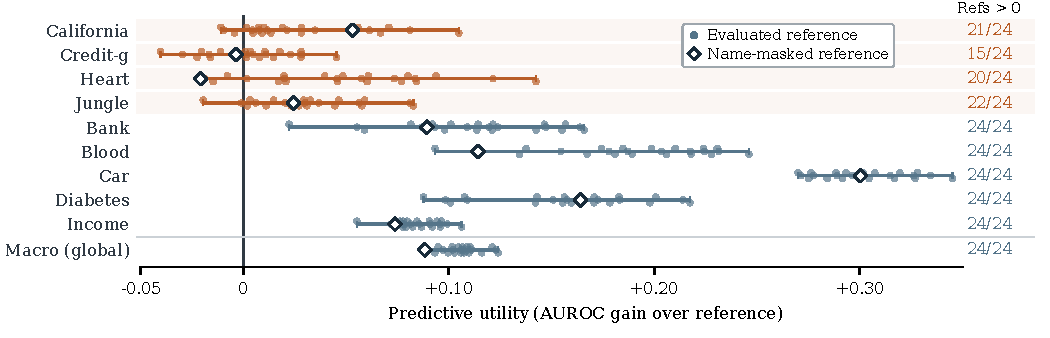
\includegraphics[width=0.90\linewidth]{figure_reference_sensitivity.pdf}
\caption{
Reference sensitivity of TabLLM predictive utility.
Points show the 24 evaluated identifier assignments, diamonds mark the primary name-masked reference, and horizontal lines show the point-estimate range; orange rows indicate ranges that cross zero.
Counts at right show the number of positive estimates.
}
\label{fig:ref_sensitivity}
\end{figure}

Across datasets, $79.2-99.7\%$ of the variation across references remains after accounting for evaluation noise with paired resampling over shared test rows.
Only for Jungle do simultaneous 95\% confidence bands confirm a sign change, with one band entirely below zero and another entirely above zero.
The other three crossings rest on point estimates only and remain unresolved.
Reference choice clearly affects utility magnitude, while evidence that it changes the resolved sign is much more limited.
Reference-dependent variation remains when we restrict the analysis to the four datasets whose published TabLLM results we reproduce most closely. 
Similar variation also appears with alternative generic identifier labels, although zero crossings are less frequent.
Satisfying the reference criteria allows predictive utility to be estimated, but different suitable references can still yield different values.
We recommend reporting reference sensitivity when multiple suitable references are available.

\subsection{Predictive Utility Depends on What the Reference Can Recover}
\label{sec:reference_recover}

We next test this dependence in two complementary ways: making the tested information harder to recover from observed inputs and easier to recover from labeled target examples.
As a real-data reference point, measurement knowledge has positive utility across 10 clinical endpoints ($+.197$, 95\% CI $[+.110,+.294]$).

\paragraph{Utility increases when information is harder to recover from observed inputs.}

In the controlled benchmark, we test how measurement utility changes as source--target measurement mismatch increases, making the required transformation harder for the reference to infer.
For relation knowledge, we instead remove constituent inputs, making the supplied relation value harder to recompute.
Within each comparison, the intended and reference conditions receive the same observed inputs \supp{\S\ref{sec:app-measurement-dose}, \S\ref{sec:app-relation-value-interface}}.
Across both interventions, utility increases as the tested information becomes harder to recover.
At the largest measurement mismatch and $n_{\mathrm{target}}=32$, XGB utility reaches $+.259$ to $+.260$ across the three target structures.
Relation utility similarly rises from $+.002$ to $+.242$ as the constituent inputs are removed.
This increase comes mainly from deterioration of the reference rather than improvement of the intended condition.
In the pairwise XGB setting, intended nMSE changes only from $.708$ to $.741$, while reference nMSE worsens from $.710$ to $.983$.

Removing constituent inputs changes the information available to the model. To test whether reconstructibility is related to utility, we add noise to the constituent inputs while keeping the number of input columns fixed.
At each nonzero noise level, lower reconstruction $R^2$ shows a modest association with higher utility (within-setting Spearman $\rho$ between $1-R^2$ and utility, averaged over eight settings at each dose: $+.165$ to $+.329$; \supp{\S\ref{sec:app-noisy-proxy}}).
Because this relationship cannot be isolated from other input changes in the real-data relation experiments, we treat it as a modest association observed in the controlled benchmark rather than a mechanism established in real-data transfer.

\begin{figure}[h]
\centering
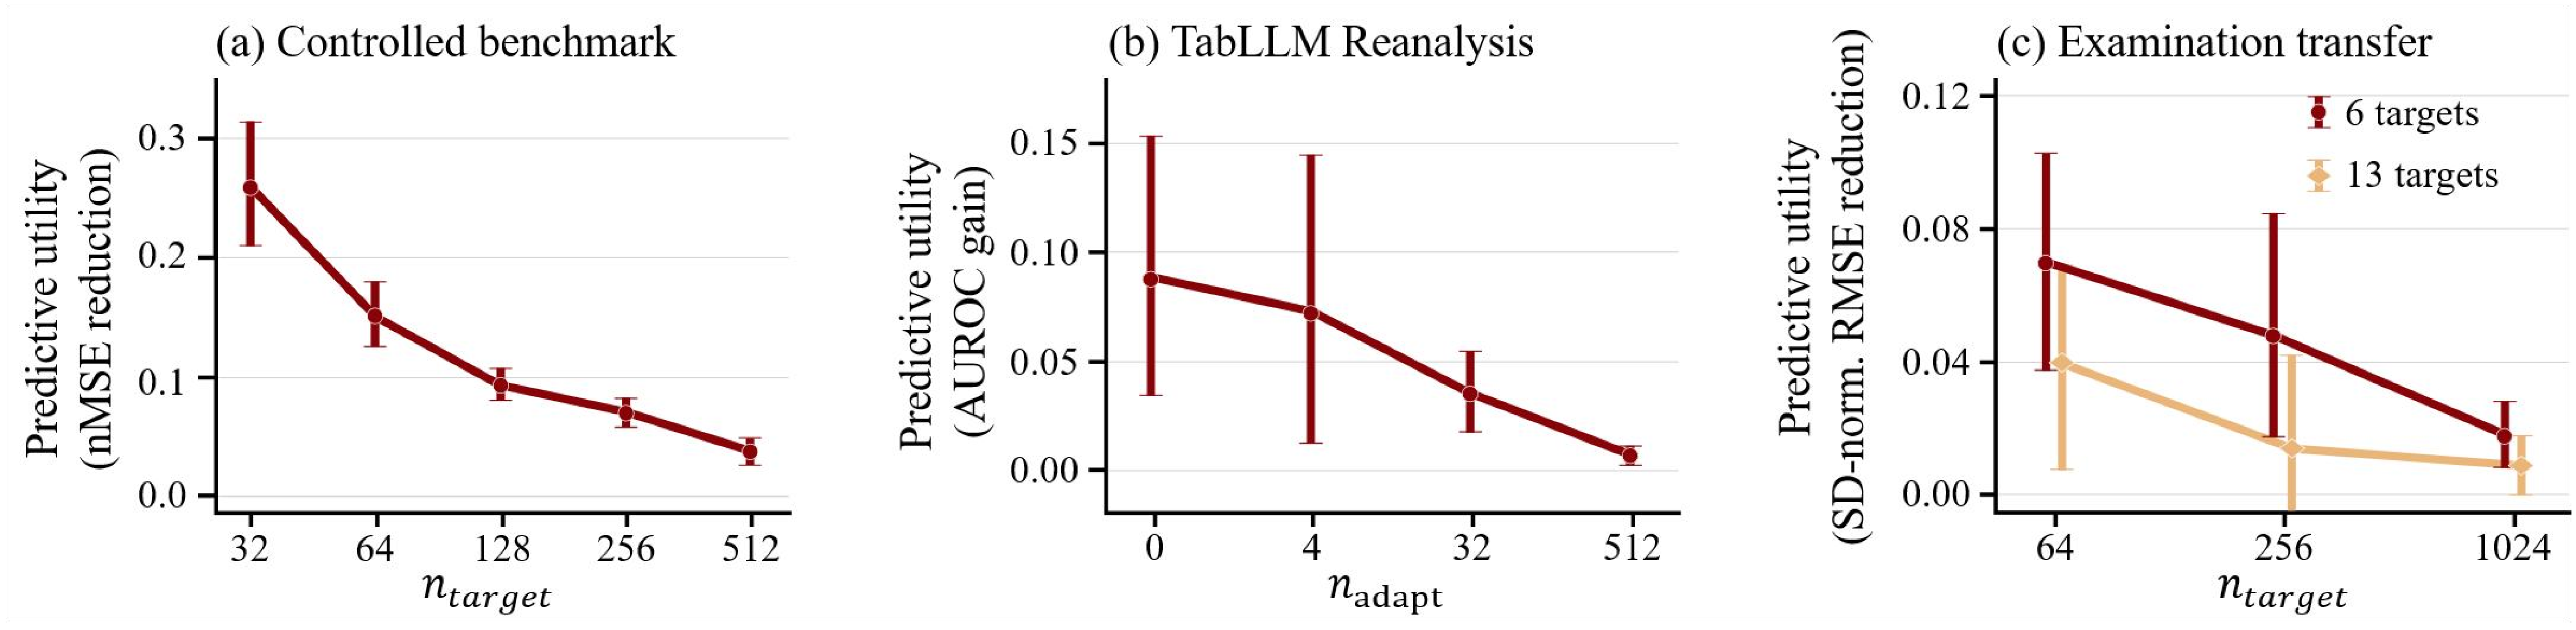
\includegraphics[width=0.95\linewidth]{figure2_real_support_reference.pdf}
\caption{
Predictive utility decreases as labeled target support increases.
\textbf{(a)} Controlled measurement-knowledge utility for pairwise XGB at the largest tested measurement mismatch.
\textbf{(b)} Mean TabLLM feature-name utility across nine datasets relative to the name-masked reference.
\textbf{(c)} Correspondence-knowledge utility across a post hoc six-endpoint subset defined by whether the target itself is a matched variable, with the full 13-endpoint trajectory shown alongside it for comparison.
Intervals are 95\% CIs; metrics differ across panels and magnitudes are not directly comparable.
}
\label{fig:real_support_reference}
\end{figure}

\paragraph{Utility decreases as labeled target support increases.}
Labeled target examples give the reference another way to recover task-relevant information.
Accordingly, utility decreases as target support increases for the continuous clinical endpoints, in TabLLM, and the controlled benchmark (Figure~\ref{fig:real_support_reference}).

Among the six examination endpoints for which the target itself is a matched variable, correspondence utility falls from $+.070$ to $+.018$ as target support increases.
This attenuation is driven mainly by the reference catching up: SD-normalized RMSE improves from $.738$ to $.676$, while the reference improves from $.808$ to $.694$.
The broader 13-endpoint analysis shows the same downward trend, although utility at $n_{\mathrm{target}}=256$ remains unresolved ($+.014$, 95\% CI $[-.013,+.042]$).

The decline extends beyond continuous clinical endpoints.
TabLLM utility falls from $+.088$ to $+.007$, a decrease of $.081$ (95\% CI $[+.025,+.148]$), and utility is lower at $n_{\mathrm{adapt}}=512$ than at $0$ under all 24 evaluated references.
In the controlled benchmark, utility at the largest measurement mismatch falls from about $+.26$ to $+.03$ across the three prespecified target structures.

Together, these results show that utility is larger when the reference has fewer ways to recover the tested information. 
Making that information harder to recover increases utility, while labeled target examples allow the reference to catch up and reduce it.
Across both manipulations, the intended condition changes comparatively little; most of the variation comes from reference performance.
The measured utility also depends on the learner; additional capacity and learner-coverage analyses are reported in \supp{\S\ref{sec:app-relation-capacity}, \S\ref{sec:app-learner-coverage}}.

\subsection{Implications for Published Semantic Ablations}
\label{sec:broader_scope}

Given this dependence on the control, we ask whether published semantic ablations use controls that match their stated predictive claims.
Using a fixed inclusion rule, we audit 25 comparisons from nine studies that alter or remove an identifiable semantic component \supp{\S\ref{sec:published_audit}}.
This is a bounded audit of claim--control alignment, not an estimate of its prevalence in the literature.
For each comparison, we record the claim and assess whether the reported control isolates the claimed effect of the tested component.
For a predictive-utility claim, the control must remove the tested semantic component while preserving the remaining information, input interface, model, and learning procedure.
We classify the comparison as supported when all three requirements hold, unsupported when at least one clearly fails, and indeterminate when the published description is insufficient to establish them.

\begin{table}[!ht]
\centering
\vspace{-0.4em}

\caption{Claim--control alignment in the published-ablation audit.}
\label{tab:published_audit}
\vspace{0.1em}

\fontsize{8pt}{9pt}\selectfont
\setlength{\tabcolsep}{3pt}
\renewcommand{\arraystretch}{0.95}

\begin{tabular}{@{}lccc@{}}
\toprule
Claim type & Supported & Unsupported & Indeterminate \\
\midrule
Content sensitivity ($n=4$) & 3 & 1 & 0 \\
Predictive utility ($n=18$) & 1 & 11 & 6 \\
\bottomrule
\end{tabular}

\vspace{1pt}

{\scriptsize \emph{*Note.*} A comparison may make both claim types, so the rows are not mutually exclusive.
Counts include explicit claims only; for predictive utility, 18 comparisons make an explicit claim, five make no claim, and two have unclear scope.}

\vspace{-0.5em}
\end{table}

Among the 18 explicit predictive-utility claims, only one is paired with a control that satisfies all three requirements; 11 fail at least one requirement, and six cannot be determined from the published description.
Thus, most controls in this bounded sample do not by themselves isolate the predictive utility claimed for the tested semantic component.
Importantly, this does not show that the reported semantic knowledge is unhelpful.
It means only that the reported comparison does not isolate predictive utility under our criteria.
% The assessment is comparison-specific rather than study-specific.
% For example, in ConTextTab, C08-A--D fail Preservation, whereas C08-E remains indeterminate because the published description does not establish whether the same learning procedure was used.

Because these judgments require manual coding, we also examined agreement between the two coders.
Preservation had the lowest agreement in the initial coding ($\kappa=.265$; \supp{\S\ref{sec:published_audit}}).
We therefore replaced the broad Preservation judgment with six fixed checks, after which the same two coders independently re-coded all 25 comparisons before reviewing disagreements.
Accordingly, the audit evaluates what each reported control can identify for the stated claim, rather than judging the overall correctness of the study or method.

\section{Conclusion}

Sensitivity to altered semantics does not by itself quantify the predictive contribution of semantic knowledge in cross-table transfer.
Across our analyses, predictive utility depends on the reference, the information available without the tested knowledge, labeled target support, and the model straining setup.
Altered controls remain informative: they can show whether prediction depends on the supplied semantic content, but they should not be interpreted as direct estimates of predictive utility.
Our bounded audit shows that this distinction also matters in published practice, where many reported controls do not by themselves isolate the claimed predictive utility.
These results support claim-matched evaluation: controls should be chosen for the predictive claim they support, with predictive-utility claims requiring a suitable reference and reference sensitivity reported when several are available.

\section*{Reproducibility Statement}

The supplementary material provides the experimental settings, inference procedures, analysis provenance, reference constructions, and robustness analyses required to reproduce the reported comparisons.
The public repository contains code, frozen semantic records and reference libraries, analysis manifests, environment information, and mappings from reported tables and figures to their generating scripts and outputs.
Public datasets can be obtained from their original sources; data requiring registration or license, including KNHANES and HRS, are not redistributed, and their access boundaries and reproducible derived outputs are documented in the supplement.

\section*{AI Use Statement}

Generative AI tools were used in this work in two roles.
First, language models were used in parts of the semantic-knowledge construction process to propose candidates from schema metadata and dataset documentation.
These steps did not use target labels or predictive performance, and the resulting semantic specifications were fixed before evaluation, as described in Section~\ref{sec:knowledge_construction}.
Second, generative AI tools were used during research development to provide feedback on experimental design and methodology and to assist with the interpretation of results.
They were also used during manuscript preparation for drafting, editing, organization, and formatting.
All experimental decisions, analyses, numerical results, references, and claims were reviewed and verified by the authors, who take responsibility for the final content of the work.
Generative AI tools were also used to assist with software organization, validation, and preparation of the supplementary reproducibility artifact; all AI-assisted code and artifact contents were reviewed and verified by the authors.
\bibliography{references_seed}
\bibliographystyle{iclr2027_conference}

\ifdefined\ICLRIncludeAppendix
\input{appendix.inc}
\fi

\end{document}
